\chapter{CFDDB测试集}
\label{chap:establishCFDDB}

在选择正确的算法之前,我们应当选择或者建立一套测试集,以检测算法执行的效果。在人脸检测的领域,已经有数量众多的公开数据集用于训练和测试,常见的有WIDER FACE\cite{yang2016wider},FDDB\cite{fddbTech},LFW\cite{huang2007labeled}等等。然而如图\ref{fig:chap1:pic}所示,这些数据集中的人脸大多是欧美人,而且每张照片中的人脸数量也有限。而我们从监控录像中提取的图片亚洲人偏多,人脸往往是模糊的,大角度的,或是被遮挡的。因此,现有的数据集无法满足我们的测试需求,据此我们建立了自己的数据集CFDDB(Classroom Face Detection Database)。


\begin{figure}[!htp]
	\centering
	\begin{subfigure}{6cm}
		\centering
		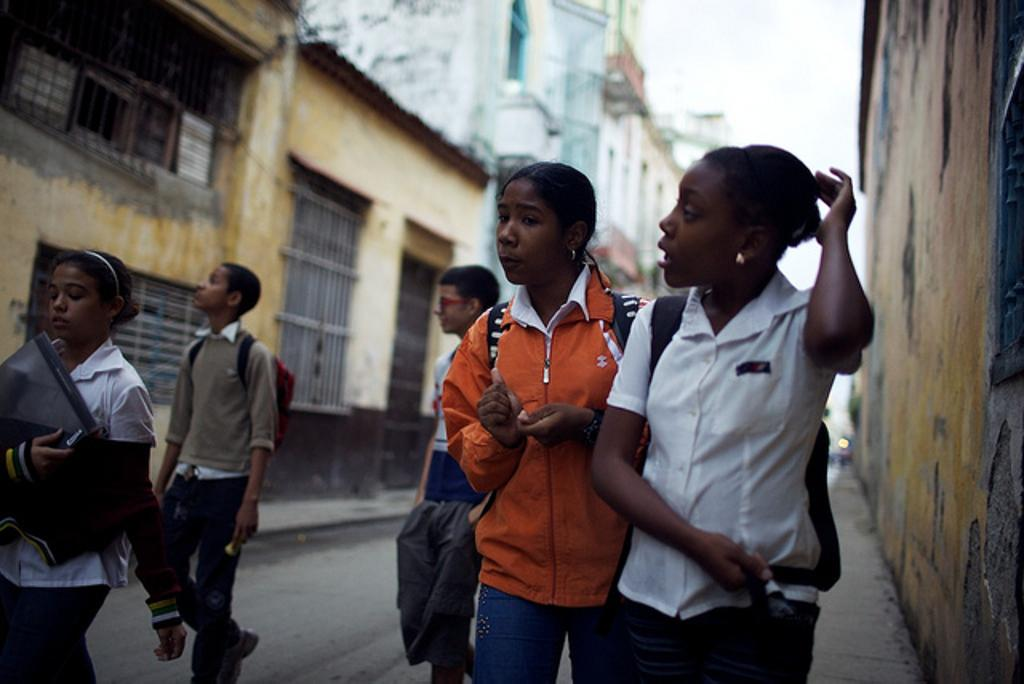
\includegraphics[width=6cm,height=4cm]{chap1/1.jpg}
		\caption{WiderFace 测试集样例图片}
	\end{subfigure}
	\hspace{4em}
	\begin{subfigure}{6cm}
		\centering
		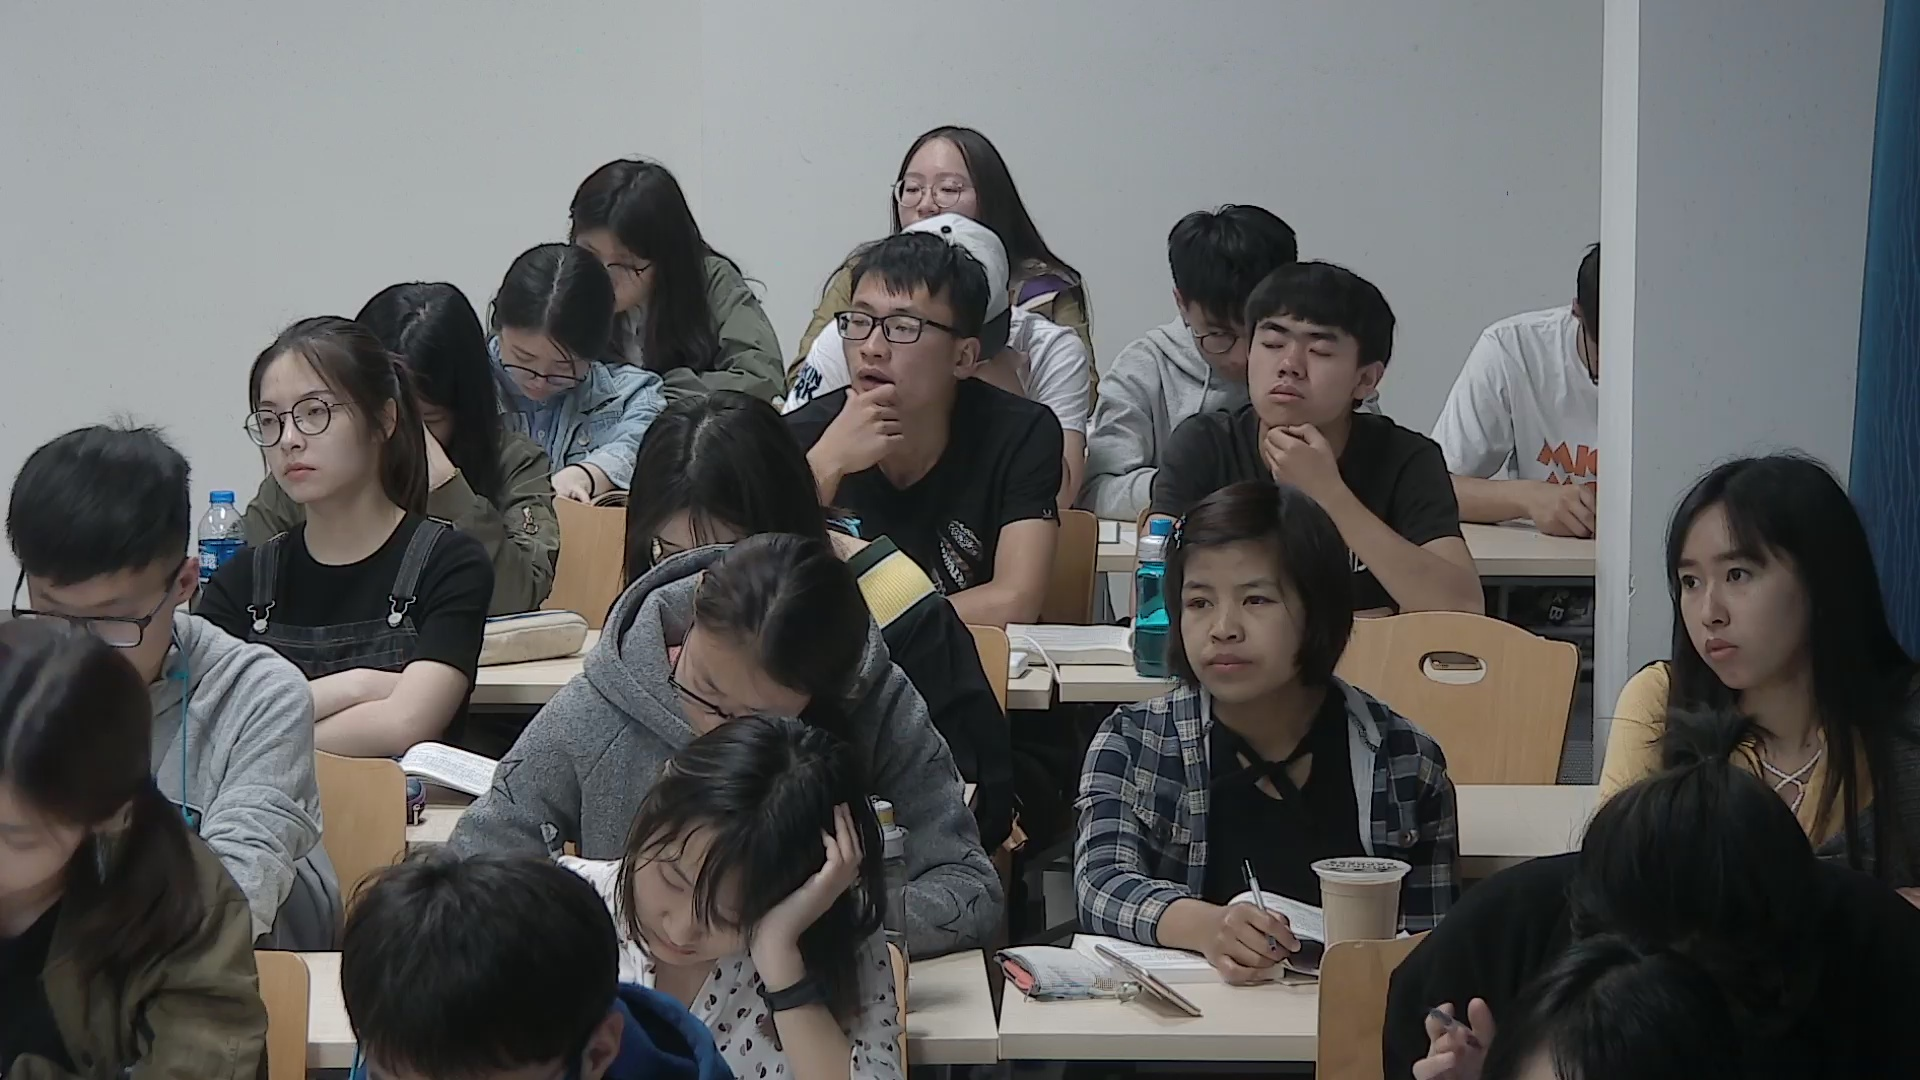
\includegraphics[width=6cm,height=4cm]{chap1/2.jpg}
		\caption{CFDDB 测试集样例图片}
	\end{subfigure}
	\bicaption{WIDER FACE与CFDDB样例图片对比图}{Sample picture comparision between WIDER FACE and CFDDB}
	\label{fig:chap1:pic}
\end{figure}


\section{CFDDB测试集图片标注规则}

测试集图片由从一段15分钟的监控录像中每隔100帧截取一帧产生,共有149张图片。标注人需要在一张图片中使用矩形框标注全部可识别人脸。标注的矩形框应当以人脸的鼻子为中心,矩形框区域面积应当大概是人脸区域面积的两倍。图\ref{fig:chap1:cfddblbexp}为CFDDB中一张图片的标注可视化之后的效果,其中,绿色的矩形框为标注人标注的人脸区域。

\begin{figure}[!htp]
	\centering
	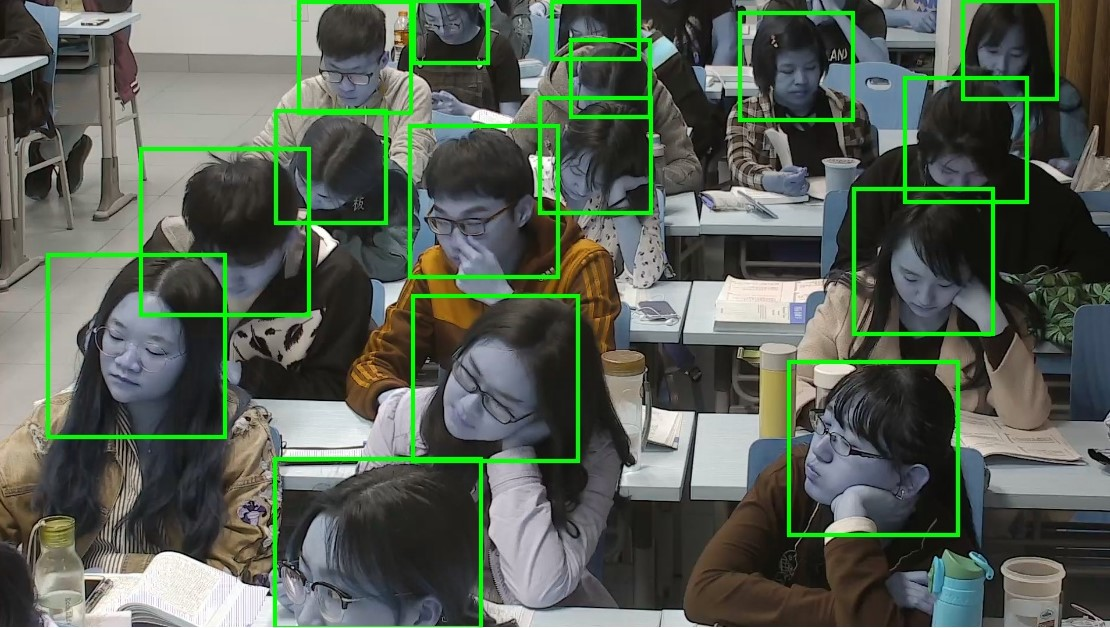
\includegraphics[height=6cm]{chap1/3.jpg}
	\bicaption{CFDDB 标注示例}{A lable example from CFDDB}
	\label{fig:chap1:cfddblbexp}
\end{figure}

矩形框标注完毕之后需要给每一个矩形框添加一个标签,这个标签是人脸的全局名称。标签添加完毕之后,将一张图片中所有矩形框的位置信息和标签信息写入与图片同名的XML文件进行保存。

为了保证视频中每位老师和同学的隐私,我们给每张人脸添加的全局标签均为一定规则生成的独特的数字组合而不是姓名,以保证数据集不被滥用。

\section{CFDDB测试集的纠错与预处理}

测试集的标注是人为进行的,有可能会出现差错,所以在将标注信息加入测试集之前,还需要对标注的信息进行认真反复的比对,以确保标注信息的正确性。在本次比对中,共发现六处错误。修改所有错误之后,测试集中共有可用图片134张,人脸1087个,总人数84人。

测试集的预处理分为四步。第一步是将所有人脸图像区域切割出来,并将相同的人脸放到以该人脸的标签为名的文件夹下。这么做的目的是方便建立之后的识别数据库,而且通过对每个文件夹中的内容的比对,可以再次检验人为标注是否准确。

第二步是对齐所有人脸。由于人为标注的人脸有大有小,所以需要将所有截出的人脸图像对齐到相同大小。CFDDB在建立时保持了原有人脸的长宽比,不足的地方以空白图像补全,之后使用线性插值的方式将所有人脸缩放到了宽150像素,高150像素的大小。

第三部是将截取出的所有人脸进行人工筛选。对于每一张图像,如果其人脸露出面积占总图像面积不超过$30\%$或者原始人脸大小的高度小于10像素的区域,则将其标记为忽略。

第四步是将所有对齐的人脸进行预识别,得到特征向量。CFDDB在建立时使用了MtCNN\cite{zhang2016joint}进行校正,使用InsightFace\cite{deng2018arcface}提取特征向量。最后,每一张截出的人脸图像都转化为了一个256维的特征向量。

最后一步是对所有抽取出的特征向量进行聚类,使用算法\ref{algo:classcenter}计算出每个类的类中心作为该人脸的标准特征向量,并保存到以该人脸标签为文件名的Numpy向量文件中。

\begin{algorithm}
	% \begin{algorithm}[H] % 强制定位
	\caption{求类中心}
	\label{algo:classcenter}
	\begin{algorithmic}[1] %每行显示行号
		\Require $Array$类成员向量数组,$n$类成员个数 % 输入
		\Ensure $center$类中心向量 % 输出
		\Function {CalcAverage}{$Array, n$}
		\State $result \gets 0$
		\For {$i = 0 \to n-1$}
		\State $result \gets result + Array[i]$
		\EndFor
		\algstore{a}
	\end{algorithmic}
\end{algorithm}

\begin{algorithm}
	\begin{algorithmic}[1]
		\algrestore{a}
		\State \Return{$result$}
		\EndFunction
		\State
		\Function{Normalize}{$vector$}
		\State $l\gets 128$
		\State $norm\gets 0$
		\For {$j = 0 \to l-1$}
		\State $norm\gets norm + vector[j] * vector[j]$
		\EndFor
		\State $norm\gets \sqrt{norm}$
		\State $norm\gets vector / norm$
		\State \Return{$norm$}
		\EndFunction
		\State
		\Function{CalcCenter}{$Array, n$}
		\State $center\gets $\Call{ClacAverage}{$Array, n$}
		\State $center\gets $\Call{Normalize}{$center$}
		\State \Return{$centor$}
		\EndFunction
	\end{algorithmic}
\end{algorithm}

\section{CFDDB测试集的使用}

CFDDB测试集既可以用来测试无感知人脸检测算法的准确性,又可以粗测无感知人脸识别算法的准确性。CFDDB中的所有内容都可以在CFDDB的Github主页\footnote{https://github.com/liuwuliuyun/CFDDB}中找到,主页中还包含了针对不同算法检测的示例程序。下面介绍如何使用CFDDB数据集:

\subsection{使用CFDDB测试人脸检测算法}

下述检测方法中$ImageList$表示CFDDB测试集的图像列表,$GroundTruth[image]$表示对应$image$图片的人为标注区域列表,$Detect[image]$表示对应$image$图片使用人脸检测算法得到的区域列表,$TargetIOU$表示人为设定的标定区域和检测区域的交叠率。检测方法如下:

\begin{enumerate}
	\item 从$ImageList$中取出待检测的图像$image$。
	\item 调用待测的检测算法得到$Detect[image]$,同时读出人为标注信息$GroundTruth[image]$。
	\item 计算$Detect[image]$中每一项与$GroundTruth[image]$中每一项的交叠率,如果最大的交叠率超过了预设的$TargetIOU$则认为成功的检测到了一张人脸。
	\item 计算所有检测到的人脸数目,并将检测错误的信息输出分析检测算法存在的缺陷。
\end{enumerate}

\subsection{使用CFDDB测试人脸识别算法}

下述检测方法中$FaceImage$表示待检测的人脸图片区域,$GroundTruth[FaceImage]$表示人为标注的人脸编号,$Recognize[FaceImage]$表示识别得出的人脸向量,$FaceList$表示经过预处理后得到的每一个人脸编号对应的类中心向量。检测方法如下:

\begin{enumerate}
	\item 取出待检测人脸区域的人为标注编号$GroundTruth[FaceImage]$。
	\item 调用人脸识别算法得到$Recognize[FaceImage]$。
	\item 计算$Recognize[FaceImage]$到$FaceList$中每一项的欧氏距离,将距离最小的一项对应的标签与$GroundTruth[FaceImage]$比对,如果相同,认为识别正确;如果不同,认为识别错误。
	\item 计算所有识别正确的人脸数目,并将错误信息输出分析识别算法存在的缺陷。
\end{enumerate}

\section{CFDDB测试参数定义}

以下三个参数均用于测试人脸检测算法的准确性,其中参数$\alpha$为结合召回率和误判率两种参数的综合测试指标。

CFDDB测试集中全部的人脸数量为$face_{all}$,检测正确的人脸数量为$face_{right}$,定义召回率$recall$为:

\begin{equation}
\label{eq:rdef}
recall = \frac{face_{right}}{face_{all}} 
\end{equation}

CFDDB测试集中全部的人脸数量为$face_{all}$,检测错误的人脸数量为$face_{wrong}$,定义误判率$errorrate$为:

\begin{equation}
\label{eq:edef}
errorrate = \frac{face_{wrong}}{face_{all}} 
\end{equation}

CFDDB测试集中召回率为$recall$,误判率$errorrate$,定义检测参数$\alpha$为:

\begin{equation}
\label{eq:alphadef}
\alpha = \frac{1}{recall} + 10\cdot errorrate
\end{equation}

\section{CFDDB测试集属性分析}

CFDDB测试集由于专注于课堂教室这个特殊的场景,适用于对教室点名的人脸识别系统进行测试,整体难度与WIDER FACE\cite{yang2016wider}的Hard测试集相当。但是,CFDDB又与WIDER FACE数据集在人脸大小、人种等属性上有着明显的差别。下面我们对CFDDB测试集做属性分析。由于CFDDB测试集是从视频流中截取的,因此我们采用平均取样的方法,从测试集中每隔20张图片选取一张作为属性分析的样本。

\subsection{大小}

我们根据人脸区域的高度将人脸分为三种大小:较大人脸,中等人脸和较小人脸。这里沿用WIDER FACE数据集中的定义,将较小人脸定义为高10像素到高50像素的人脸;将中等人脸定义为高50像素到高300像素的人脸;将较大人脸定义为高度超过300像素的人脸。

\subsection{肤色}

与WIDER FACE数据集中多种肤色的人脸不同,CFDDB中的人脸全部是肤色为黄色的亚洲人。未来可能添加包括多种肤色的图片以提供不同测试环境下的需求。

\subsection{遮挡}

遮挡在评估人脸检测算法中的表现中有着不可替代的作用。这里同样沿用WIDER FACE中的定义,将部分遮挡定义为人脸被遮挡的区域占全部人脸区域的$1\%$至$30\%$;严重遮挡定义为人脸被遮挡的区域占全部人脸区域超过$30\%$。

\subsection{姿势}

这里类比WIDER FACE中姿势的定义。若满足一下两中条件中的任意一种,则一张人脸被定义为非正脸。条件一是俯仰角超过30度。条件二为偏航角超过90度。若两个条件都不满足,则该人脸区域被定义为正脸。

\subsection{教室类型}

在这里我们定义三种不同的教室类型:大型教室、中型教室和小型教室。其中大型教室为学生数量超过100人的教室;中型教室为学生数量介于30至100人之间的教室;小型教室为学生数量少于30人的教室。目前,CFDDB中的区域仅有中等教室,后续会在CFDDB测试集的扩充中陆续添加从小型教室和大型教室获取的人脸图像与标记。

\subsection{分析结果}

对取样的到的7张图片进行分析,结果如表\ref{tab:cfddbal}所示:

由于取样的均匀性,这7张图片可以一定程度上代表整个CFDDB测试集的属性情况。从图\ref{fig:chap1:cfddb1}可以看出CFDDB中非正脸的图像占据了超过$70\%$,从图\ref{fig:chap1:cfddb3}可以看出,有遮挡人脸占比达到了$58\%$。这些特性使得CFDDB测试集对任何人脸检测算法和识别算法都是极大的挑战。

\begin{table}[!hpb]
	\centering
	\bicaption[CFDDB测试集属性]
	{CFDDB测试集属性}
	{CFDDB test dataset properties}
	\label{tab:cfddbal}
	\begin{tabular}{ c | ccccccc | c }
		\hline
		人脸属性 & 004 & 024 & 044 & 064 & 084 & 104 & 124 & 总计\\
		\hline
		较小人脸 & 0 & 0 & 0 & 0 & 0 & 0 & 0 & 0\\
		中等人脸 & 3 & 4 & 3 & 0 & 0 & 0 & 4 & 14\\
		较大人脸 & 2 & 9 & 7 & 5 & 4 & 3 & 6 & 36\\
		无遮挡   & 3 & 7 & 3 & 1 & 3 & 2 & 2 & 21\\
		部分遮挡 & 1 & 3 & 2 & 2 & 0 & 1 & 3 & 12\\
		严重遮挡 & 1 & 3 & 5 & 2 & 1 & 0 & 5 & 17\\
		正脸     & 2 & 5 & 1 & 2 & 0 & 2 & 2 & 14\\
		非正脸   & 3 & 8 & 9 & 3 & 4 & 1 & 8 & 36\\
		\hline
		总计 & 5 & 13 & 10 & 5 & 4 & 3 & 10 & 50\\
		\hline
	\end{tabular}
\end{table}

\begin{figure}[!htp]
	\centering
	\subcaptionbox{人脸姿势占比图\label{fig:chap1:cfddb1}}
	{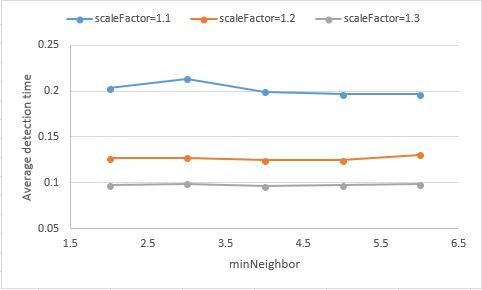
\includegraphics[height=4cm]{chap1/4.jpg}}
	\hspace{4em}
	\subcaptionbox{人脸大小占比图\label{fig:chap1:cfddb2}}
	{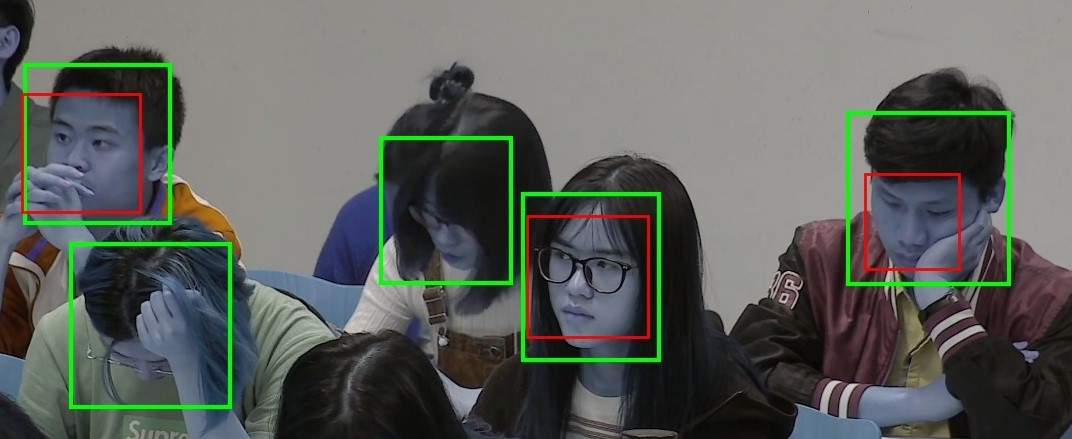
\includegraphics[height=4cm]{chap1/5.jpg}}
	\hspace{4em}
	\subcaptionbox{人脸遮挡占比图\label{fig:chap1:cfddb3}}
	{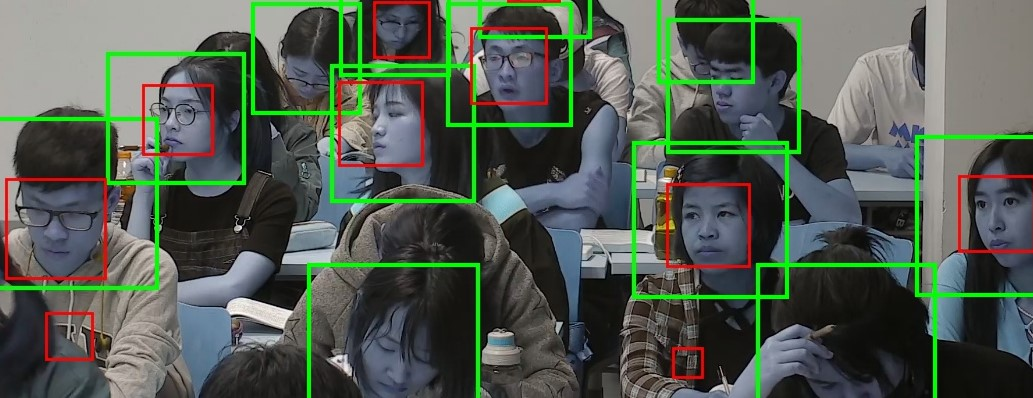
\includegraphics[height=4cm]{chap1/6.jpg}}
	\bicaption{CFDDB属性分析}{CFDDB properties analysis}
	\label{fig:cfddbeval}
\end{figure}

\section{CFDDB测试集的改进}

CFDDB由于采用了从视频流中截取连续帧的方法,使得有部分图片之间差异性较小。从而导致在测试检测算法时,如果在某张图片上效果不好,则在与之相邻的相同场景的图片上效果依然不好。这样会导致容易积累同样的错误从而使得CFDDB检测结果出现偏差。对于这种问题,可以通过使用更多的资源对数据库进行扩充来解决。如果数据量足够大,就可以稀释相似图片的积累错误,从而使得评价结果更加客观准确。

目前CFDDB采用通过剪裁截取到的图片计算类中心的方法建立人脸标准数据库。事实上这种方法只能粗略测得识别算法的准确性。更符合无感知检测场景的方法应当是由视频中出现人物的一张或多张证件照提取人脸特征向量,在对这些向量求类中心之后,得到人脸标准数据库中的人脸特征信息。目前受限于隐私保护,尚无法获得数据库中出现人脸的证件信息。这个问题有两种解决方法。第一种方法为招募志愿者,并提供完整的隐私保护政策,收集证件的照片信息。第二种方法为与受信任的机构合作,例如学校、医院,在学生或员工同意的情况下请机构提供证件的照片信息。

\section{CFDDB测试集的扩充}

限于人力和物力,CFDDB测试集目前数据量并不多。但是CFDDB在建立时就为可扩展性提供了广泛的支持。

首先,在标注人脸信息是使用了开源的工具labelImg\footnote{https://github.com/tzutalin/labelImg}与通用的XML模板。这使得即使对CFDDB测试集没有过多了解的人也可以非常容易的参与到CFDDB测试集的扩充中。其次,我们收集了多种教室类型的视频数据,并设计了开源的抽取程序,使得任何人都可以非常简单的按照与我们同样的标准抽取视频数据,在保证测试集数据一致性的基础上提升了效率。最后,我们提供了开源的XML处理程序和算法测试样例,方便更多的研究者参与和使用CFDDB数据集。

未来更多人有望能够参与到CFDDB的使用和扩充中,使得CFDDB可以成为特定场景的非受控无感知人脸检测和识别的先进测试集。如果数据量继续增加到数万张标记图片的规模,则可以将CFDDB中的数据按照某种合理的方式分为测试集和训练集,以方便对针对非受控无感知环境下人脸检测和识别算法的训练。
